%% !TEX program = xelatex
%% !BIB program = bibtex
\documentclass[10pt,aspectratio=169]{beamer}  % present

\mode<presentation>
{
    \usetheme{default}   % or try Boadilla, boxes, Singapore, Darmstadt, Madrid, Warsaw, ...
    \usecolortheme{default} % or try albatross, beaver, crane, ...

    \usefonttheme{structurebold}  % or try serif, , ...
    \setbeamertemplate{navigation symbols}{}
    \setbeamertemplate{caption}[numbered]
    \definecolor{MyColor}{rgb}{0,0.3,0.65}
    \definecolor{MyColorLight}{rgb}{0,0.7,0.95}
    \definecolor{MyGreenColor}{rgb}{0,0.6,0}
    \definecolor{MyRedColor}{rgb}{0.8,0,0}
    \setbeamercolor{structure}{fg=MyColor}
}

%% Packages
\usepackage[round]{natbib}
%\usepackage{authblk}
\usepackage{amsfonts,amsmath,amssymb,mathtools,marvosym,amsthm,ulem,cancel}
%\usepackage{enumerate}
\usepackage{graphicx,float,tcolorbox}
\hypersetup{colorlinks,linkcolor=MyColor,citecolor=MyColor,urlcolor=black,breaklinks=true}
% \usepackage{fontspec}
% \usepackage{tikz}

%% Print author name, short title, date and slide number at the bottom of the page
% \setbeamercolor{author in head/foot}{fg=MyColor, bg=MyColorLight}
\makeatletter
\setbeamertemplate{footline}
{
    \leavevmode%
    \hbox{%
        \begin{beamercolorbox}[wd=.333333\paperwidth,ht=2.25ex,dp=1ex,center]{author in head/foot}%
            \usebeamerfont{author in head/foot}\insertshortauthor
        \end{beamercolorbox}%
        \begin{beamercolorbox}[wd=.333333\paperwidth,ht=2.25ex,dp=1ex,center]{title in head/foot}%
            \usebeamerfont{title in head/foot}\insertshorttitle
        \end{beamercolorbox}%
        \begin{beamercolorbox}[wd=.333333\paperwidth,ht=2.25ex,dp=1ex,right]{date in head/foot}%
            \usebeamerfont{date in head/foot}\insertshortdate{}\hspace*{2em}
            \insertframenumber{} / \inserttotalframenumber\hspace*{2ex}
        \end{beamercolorbox}%
    }%
    \vskip0pt%
}
\makeatother

% \setmainfont{Ubuntu}
% \setmainfont{DejaVu Serif}
% \setsansfont{Segoe UI}
% \setsansfont{EB Garamond}
% \setsansfont{Tahoma}
% \setsansfont{Roboto}
% \setsansfont{Open Sans}
% \setsansfont{Georgia}
% \setsansfont{SF Pro Display}
% \setsansfont{Lato}
% \setmonofont{Monospaced}


%\setlength{\parindent}{0.5cm}
\setlength{\parskip}{0.3cm}

\renewcommand{\baselinestretch}{1.0}
\renewcommand{\arraystretch}{1.2}

\newtheorem{proposition}{Proposition}

% ------------------------------------------------------------------------------

%% Description
\author[Narek Ohanyan]{Narek Ohanyan}
\title[Lecture 5. Cointegration, Error-Correction Models]{Lecture 5. Cointegration, Error-Correction Models}
\institute[AUA]{American University of Armenia}
\date{\today}

% ------------------------------------------------------------------------------

%% Add table of contents before every subsection
\AtBeginSection[]
{
    \begin{frame}{Outline}
        \tableofcontents[currentsection]
    \end{frame}
}

% ==============================================================================

\begin{document}

\begin{frame}
    \titlepage
\end{frame}

% ==============================================================================

\section{Cointegration}

% ------------------------------------------------------------------------------

\begin{frame}{Cointegration}

    \bigskip
    Two $ \mathrm{I}(1) $ time series $ y_{t} $ and $ x_{t} $ are said to be \textbf{cointegrated} if some linear combination of them is $ \mathrm{I}(0) $.

    That is
    \begin{align*}
        y_{t} \sim \mathrm{I}(1) \qquad x_{t} \sim \mathrm{I}(1) \qquad \text{and} \quad \quad z_{t} = c_0 + c_1 y_{t} + c_2 x_{t} \qquad z_{t} \sim \mathrm{I}(0).
    \end{align*}
    for some constants $ c_0, c_1, c_2 $.

    \medskip
    Cointegration implies that $ y_{t} $ and $ x_{t} $ share \textbf{similar} stochastic trends and \textit{never diverge} too far from each other.

    \medskip
    In other words, cointegration implies that the two series are \textit{not independent}, but rather \textbf{move together} in the long run.

\end{frame}

% ------------------------------------------------------------------------------

\begin{frame}{Testing for cointegration}

    \bigskip
    The most common test for cointegration is the \textbf{Engle-Granger} two-step procedure.

    \begin{enumerate}\itemsep=1em
        \item Estimate the cointegrating regression
              \begin{align*}
                  y_{t} = \alpha + \beta x_{t} + e_{t}.
              \end{align*}
              and obtain the residuals $ \widehat{e}_{t} $.

        \item Test the residuals $ \widehat{e}_{t} $ for stationarity using the ADF test.
    \end{enumerate}

    \medskip
    If the residuals are \textbf{stationary}, then the two series are \textbf{cointegrated}.

    \medskip
    The test is based on the following regression
    \begin{align*}
        \Delta \widehat{e}_{t} = \gamma \widehat{e}_{t-1} + e_{t}.
    \end{align*}

\end{frame}

% ------------------------------------------------------------------------------

\begin{frame}{Critical values for cointegration test}

    \bigskip
    \begin{figure}[H]
        \centering
        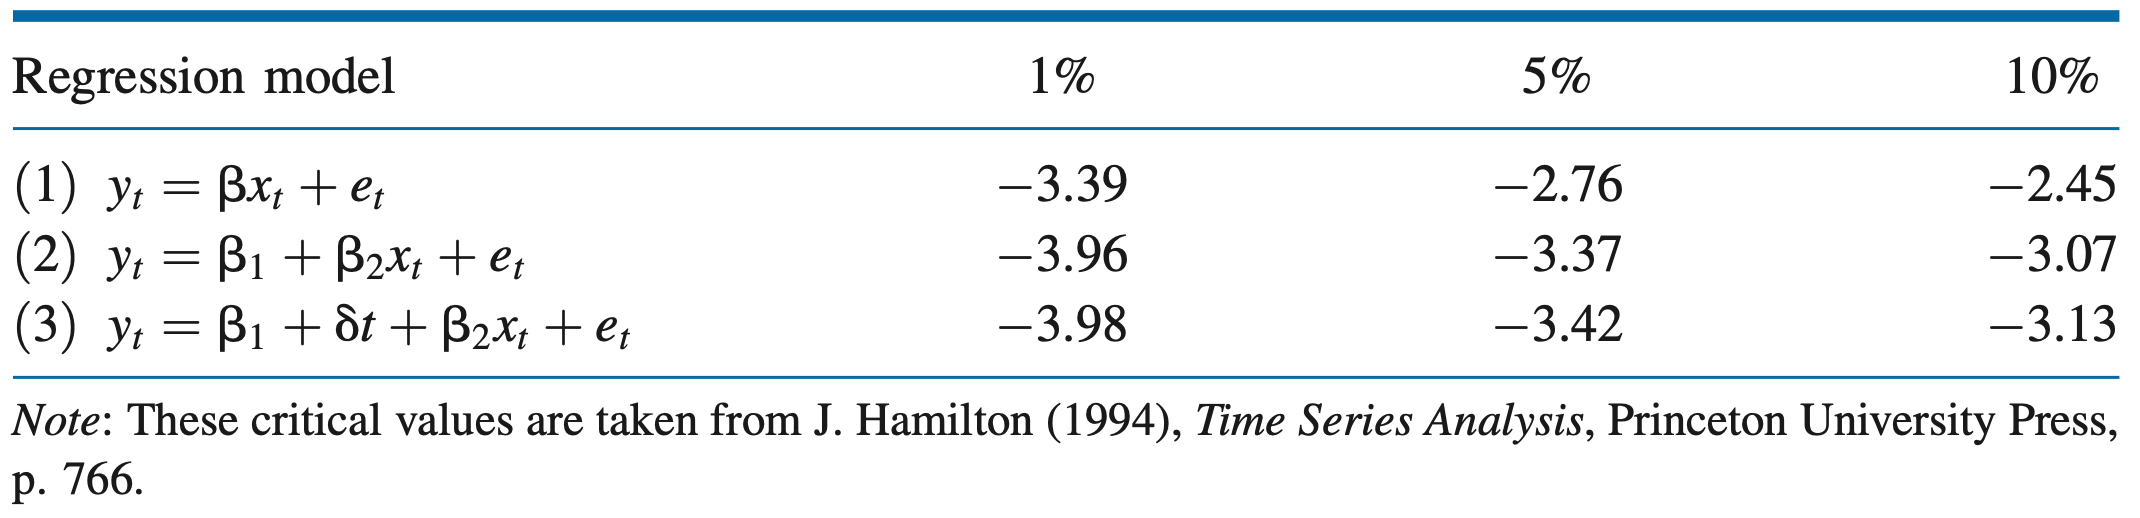
\includegraphics[height=0.2\textwidth]{./fig/engel-granger-critical-values.png}
    \end{figure}

\end{frame}

% ==============================================================================

\section{Error-Correction Models}

% ------------------------------------------------------------------------------

\begin{frame}{ARDL model with cointegrated variables}

    \bigskip
    Consider an ARDL(1,1) model of the form
    \begin{align*}
        y_{t} & = \delta + \phi_1 y_{t-1} + \delta_0 x_{t} + \delta_1 x_{t-1} + e_{t}.
    \end{align*}
    where $ y_{t} $ and $ x_{t} $ are \textbf{cointegrated}.

    \medskip
    If $ y_{t} $ and $ x_{t} $ are cointegrated, then there is a \textbf{long-run} relationship between them.

    \medskip
    The long-run relationship can be obtained by setting $ y_{t} = y_{t-1} = y $, $ x_{t} = x_{t-1} = x $, and $ e_{t} = 0 $.

    \medskip
    Then the implied long-run relationship is
    \begin{align*}
        y & = \beta_0 + \beta_1 x
    \end{align*}
    where $ \beta_0 = \delta / (1 - \phi_1) $ and $ \beta_1 = (\delta_0 + \delta_1) / (1 - \phi_1) $.

\end{frame}

% ------------------------------------------------------------------------------

\begin{frame}{Error-correction model (ECM)}

    \bigskip
    Recall that $ y_{t} $ and $ x_{t} $ are related by an ARDL(1,1) model
    \begin{align*}
        y_{t} & = \delta + \phi_1 y_{t-1} + \delta_0 x_{t} + \delta_1 x_{t-1} + e_{t}.
    \end{align*}

    Subtracting $ y_{t-1} $ from both sides of the equation and adding $ \pm \delta_0 x_{t-1} $
    \begin{align*}
        y_{t} - y_{t-1} & = \delta + (\phi_1 - 1) y_{t-1} + \delta_0 \left( x_{t} - x_{t-1} \right) + \left( \delta_0 + \delta_1 \right) x_{t-1} + e_{t}.
    \end{align*}

    Then we can write the equation as
    \begin{align*}
        \Delta y_{t} & = \left( \phi_1 - 1 \right) \left( \frac{\delta}{1 - \phi_1} + y_{t-1} + \frac{\delta_0 + \delta_1}{1 - \phi_1} x_{t-1} \right) + \delta_0 \Delta x_{t} + e_{t}.
    \end{align*}
    or
    \begin{align*}
        \Delta y_{t} & = \alpha \left( y_{t-1} - \beta_0 - \beta_1 x_{t-1} \right) + \delta_0 \Delta x_{t} + e_{t}.
    \end{align*}

\end{frame}

% ------------------------------------------------------------------------------

\begin{frame}{Error-correction model (ECM)}

    \bigskip
    The \textbf{Error-correction model (ECM)} is given by
    \begin{align*}
        \Delta y_{t} & = \alpha \left( y_{t-1} - \beta_0 - \beta_1 x_{t-1} \right) + \delta_0 \Delta x_{t} + e_{t} \\
        & = \alpha e_{t-1} + \delta_0 \Delta x_{t} + e_{t}.
    \end{align*}
    where $ \alpha < 0 $ is the \textit{speed of adjustment} and $ \beta_0 $ and $ \beta_1 $ are the \textit{long-run coefficients}.

    \medskip
    The ECM has three important features:
    \begin{itemize}\itemsep=0.5em
        \item It allows for an underlying or \textit{fundamental (long-run)} link between variables
        \item It allows for \textit{short-run adjustments} between variables towards the long-run equilibrium
    \end{itemize}

    In practice, the ECM is estimated in two steps:
    \begin{enumerate}
        \item Estimate the long-run relationship
        \item Estimate the short-run dynamics
    \end{enumerate}

\end{frame}

% ==============================================================================

\section{Regression with No Cointegration}

% ------------------------------------------------------------------------------

\begin{frame}{Regression with No-Cointegration}

    \bigskip
    If $ y_{t} $ and $ x_{t} $ are \textbf{not cointegrated}, then regression of $ y_{t} $ on $ x_{t} $ is susceptible to \textit{spurious regression}.

    \medskip
    In this case, the relationship between $ y_{t} $ and $ x_{t} $ may be estimated by transforming the variables to stationary form.

    \medskip
    Variables can be transformed to stationary form by
    \begin{itemize}\itemsep=1em
        \item taking \textit{first differences} if the variables are \textit{difference stationary} or $ \mathrm{I}(1) $
        \begin{align*}
            \Delta y_{t} = y_{t} - y_{t-1} \qquad \Delta x_{t} = x_{t} - x_{t-1}.
        \end{align*}
        \item \textit{detrending} the variables if the variables are \textit{trend stationary}
        \begin{align*}
            \widetilde{y}_{t} = y_{t} - \alpha_1 - \delta_1 t \qquad \widetilde{x}_{t} = x_{t} - \alpha_2 - \delta_2 t.
        \end{align*}
    \end{itemize}

\end{frame}

% ------------------------------------------------------------------------------

\begin{frame}{Regression with first differences or detrended variables}

    \bigskip
    In a stationary form, the relationship between $ y_{t} $ and $ x_{t} $ can be estimated as an ARDL model
    \begin{itemize}
        \item with \textit{first differences} if the variables are \textit{difference stationary}
        \begin{align*}
            \Delta y_{t} & = \alpha + \phi_1 \Delta y_{t-1} + \beta_0 \Delta x_{t} + \beta_1 \Delta x_{t-1} + e_{t}.
        \end{align*}
        \item with \textit{detrended} variables if the variables are \textit{trend stationary}
        \begin{align*}
            \widetilde{y}_{t} & = \alpha + \phi_1 \widetilde{y}_{t-1} + \beta_0 \widetilde{x}_{t} + \beta_1 \widetilde{x}_{t-1} + e_{t}.
        \end{align*}
    \end{itemize}

    \medskip
    Alternatively, if both $ y_{t} $ and $ x_{t} $ are \textit{trend stationary}, a \textit{time trend} may be included in the regression
    \begin{align*}
        y_{t} & = \alpha + \delta t + \phi_1 y_{t-1} + \beta_0 x_{t} + \beta_1 x_{t-1} + e_{t}.
    \end{align*}

\end{frame}

% ------------------------------------------------------------------------------

\begin{frame}{Regression with non-stationary variables}

    \bigskip
    \begin{figure}[H]
        \centering
        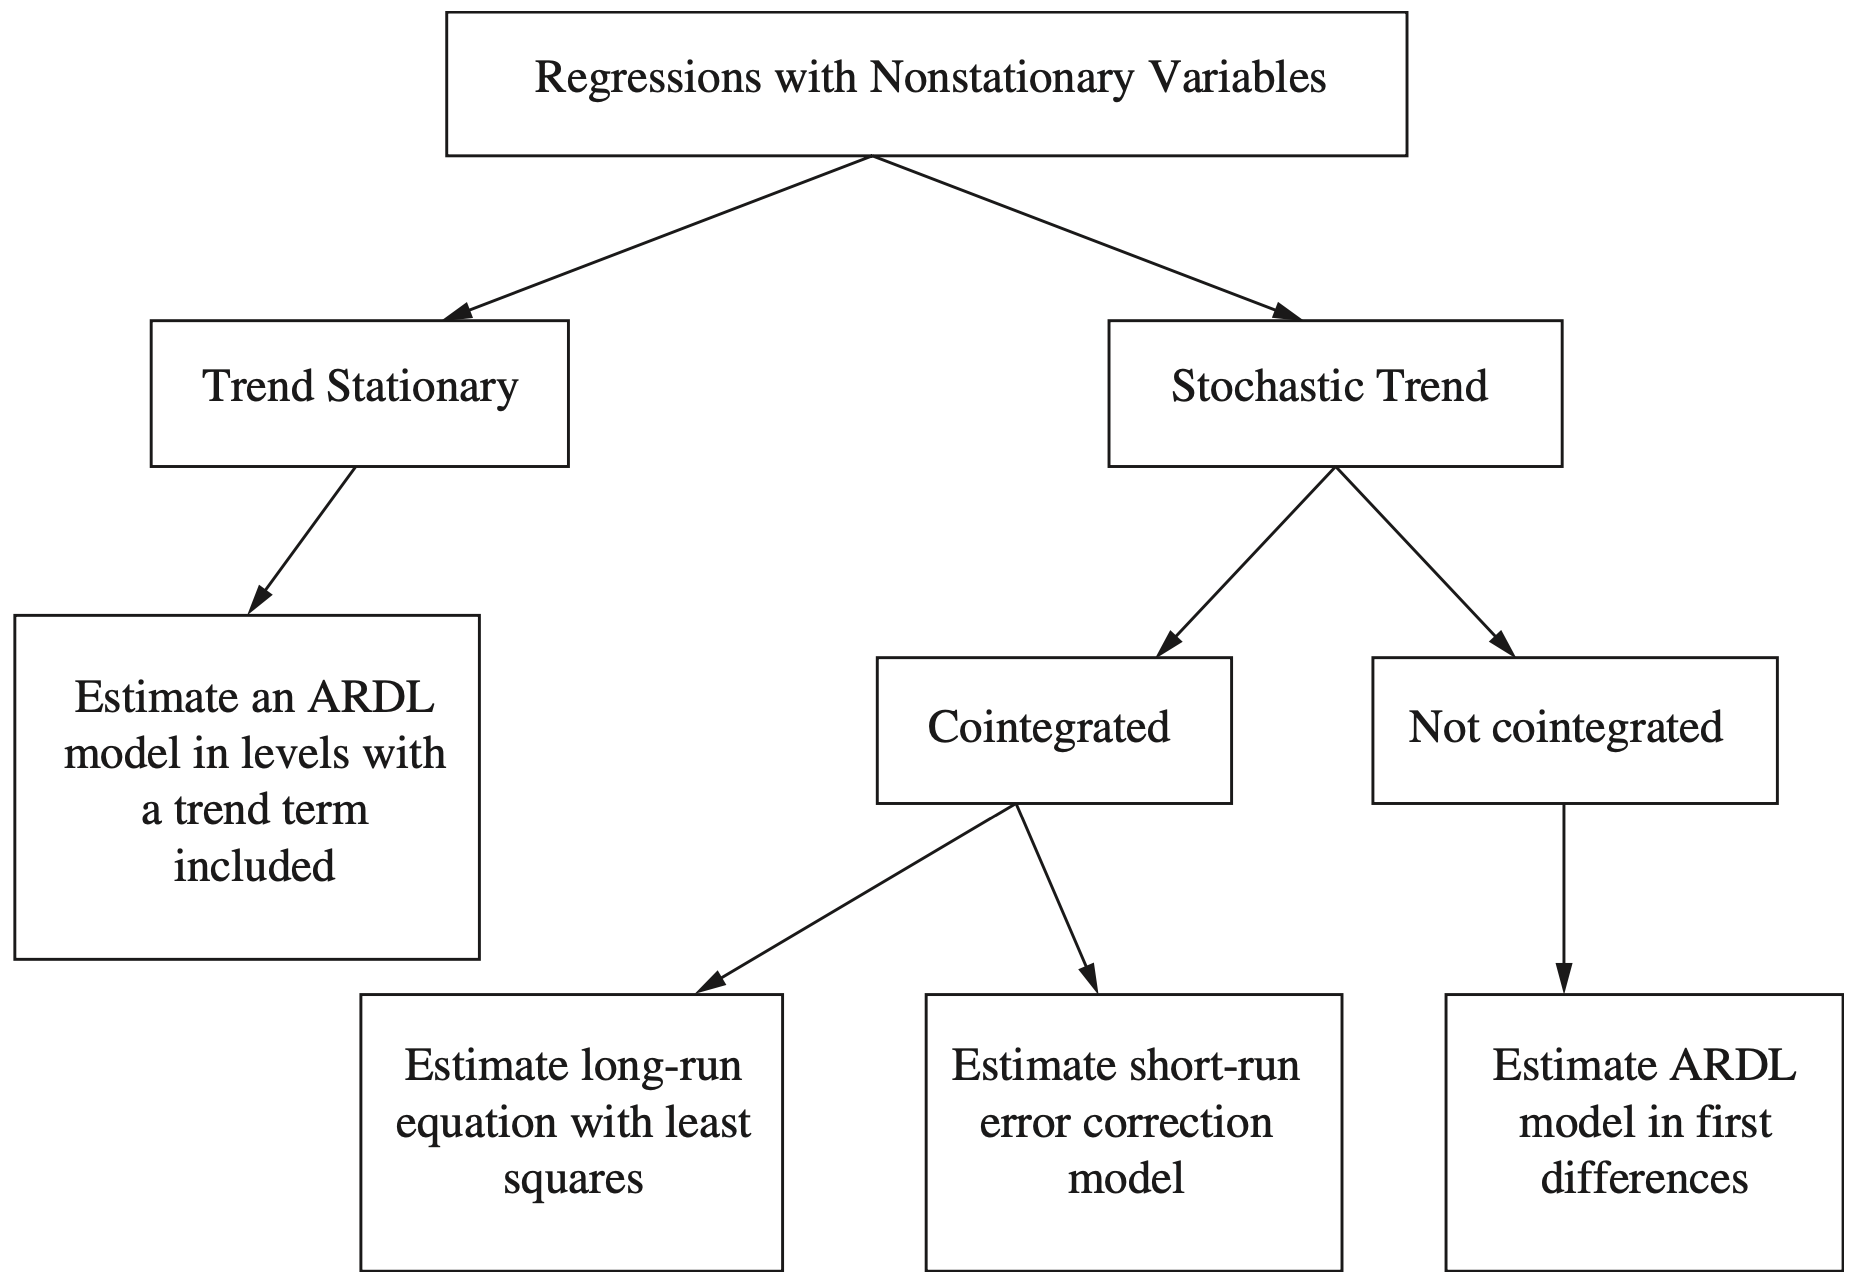
\includegraphics[height=0.5\textwidth]{./fig/regression-with-non-stationary-variables.png}
    \end{figure}

\end{frame}

% ==============================================================================

% % \begin{frame}<beamer:0>
% \begin{frame}[allowframebreaks]{Bibliography}

%     \bibliographystyle{apalike}
%     \bibliography{references}

% \end{frame}

% ==============================================================================

\end{document}
